\nsecbegin{Ziel des Sprints}
Dieser Sprint ist ausschließlich dazu gedacht, im Verlauf des ersten Sprints identifizierte und noch nicht behobene Bugs zu entfernen. Es wurden bewusst keine neuen User-Stories (für den Benutzer) im Sprint-Backlog definiert. Der Fokus liegt darauf, die im ersten Sprint geschaffene Basis noch einmal zu stabilisieren.

\nsecbegin{User-Stories des Sprint-Backlogs}
\nsecbegin{Reduzierung von Bugs}
Als Softwarearchitekt und Product Owner wünschen wir uns, dass möglichst wenige Bugs auftreten, um die spätere Weiterentwicklung und damit die uneingeschränkte Funktionalität des Produkts nicht zu gefährden.
\nsecend
\nsecend % {User-Stories des Sprint-Backlogs}

\nsecbegin{Zeitliche Planung}
\begin{figure}[hbtp]
\centering
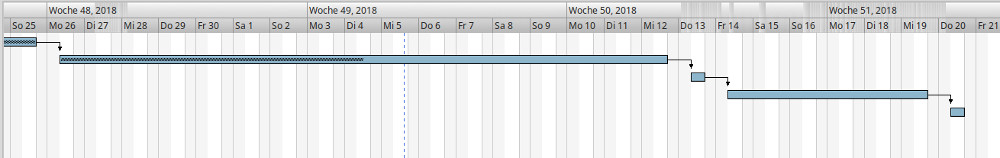
\includegraphics[width=\textwidth]{Bilder/gantt}
\caption{Gantt-Diagramm für Sprint 1}
\end{figure}
\nsecend%Zeitliche Planung

\nsecbegin{Liste der durchgeführten Meetings}
\begin{itemize}
\item Planning-Meeting (00.00.2019)
\item Zwischen-Meeting (00.00.2019)
\item Review-Meeting (00.00.2019)
\end{itemize}
\nsecend%Liste der durchgeführten Meetings

\nsecbegin{Ergebnisse des Planning-Meetings}
Der zweite Sprint wird zeitlich in der letzten Woche der Semesterferien begonnen und bis zum Ende der ersten Woche der Vorlesungszeit gehen. Dies wurde mit den Teammitgliedern besprochen. Hauptziel des Sprints ist ein sauberer Stand, mit dem ab dem kommenden Sommersemester weitergearbeitet werden kann.
\nsecend

\nsecbegin{Aufgewendete Arbeitszeit pro Person$+$Arbeitspaket}
\begin{longtable}{|p{4cm}|l|l|l|l|l|}
        \hline
        Arbeitspaket & Person & Start & Ende & h & Artefakt\\
        \hline
        Dummyklassen & Musterstudi & 3.5.09 & 12.5.09 & 14 & Klasse.java\\ \hline
        AP XYZ &  &  &  & & \\ \hline
\end{longtable}     
\nsecend

\nsecbegin{Konkrete Code-Qualität im Sprint}
Die Code-Qualität wurde durch den Fokus auf die Behebung bestehender Bugs verbessert.
\nsecend%Konkrete Code-Qualität im Sprint

\nsecbegin{Konkrete Test-Überdeckung im Sprint}
Die Test-Überdeckung in diesem Sprint war überdurchschnittlich.
\nsecend%Konkrete Test-Überdeckung im Sprint

\nsecbegin{Ergebnisse des Reviews}
\begin{table}[H]

\begin{tabularx}{\textwidth}{ |l|l|X| }
\hline
\textbf{Klasse} & \textbf{Methode} & \textbf{Anmerkungen}\\
 \hline
%Console & showConsole & Pfad anpassen \\
\hline
\end{tabularx}
\end{table}

\nsecend%Ergebnisse des Reviews

\nsecbegin{Ergebnisse der Retrospektive}
Die Retrospektive schloss mit einer positiven Bilanz. (...)
\nsecend%Ergebnisse der Retrospektive

\nsecbegin{Abschließende Einschätzung des Product-Owners}
In diesem Sprint wurden einige kritische Bugs behoben und somit User Stories des letzten Sprint-Backlogs noch vervollständigt. Zu hoffen bleibt trotzdem, dass in allen folgenden Sprints auch neue Funktionalität hinzugefügt wird.
\nsecend%Abschließende Einschätzung des Product-Owners

\nsecbegin{Abschließende Einschätzung des Software-Architekten}
XXX
\nsecend%Abschließende Einschätzung des Software-Architekten

\nsecbegin{Abschließende Einschätzung des Team-Managers}
Insgesamt kann positiv herausgehoben werden, dass sich die Teammitglieder geschlossen dazu bereit erklärten, Teil ihrer Semesterferien für den zweiten Sprint zu opfern. Die Motivation, das Produkt weiter voranzubringen, scheint derzeit ungebrochen.
\nsecend%Abschließende Einschätzung des Team-Managers